\documentclass{beamer}[10]

\usepackage{graphicx}
\usepackage{xcolor}
\usepackage{tabto}
%\usepackage{beamerthemesplit}
\usepackage{tikz}
\usepackage{cancel}
\usepackage{verbatim}
\usepackage{fancybox}
\usepackage{enumerate}
\usepackage{amsmath,amssymb,amsthm,textcomp,mathtools}
\usepackage[super]{nth}
\usepackage[amssymb]{SIunits}
\usepackage{booktabs}
\usepackage{cancel}
\usepackage{bm}
\usepackage[utf8]{inputenc}
\usepackage{tabularx}
\usepackage{ragged2e}
\newcolumntype{Y}{ >{\RaggedRight\arraybackslash}X}
\usetikzlibrary{arrows,shapes}
\newcommand\T{\rule{0pt}{2.6ex}}
\newcommand\B{\rule[-1.2ex]{0pt}{0pt}}
\definecolor{UUcrimson}{RGB}{204,0,0}
\mode<presentation>
{ \usetheme{default}
  \usecolortheme[named=UUcrimson]{structure}
  \useinnertheme{circles}
  \setbeamercovered{transparent}
  \setbeamertemplate{blocks}[rounded]
  \usefonttheme[onlymath]{serif}
  \setbeamertemplate{navigation symbols}{}
  \setbeamertemplate{footline}[page number]
  \setbeamertemplate{navigation symbols}{}
  \setbeamercolor{section in toc}{fg=black,bg=white}
  \setbeamercolor{alerted text}{fg=UUcrimson!80!gray}
  \setbeamercolor*{palette primary}{fg=white,bg=UUcrimson}
  \setbeamercolor*{palette secondary}{fg=UUcrimson!70!black,bg=gray!15!white}
  \setbeamercolor*{palette tertiary}{bg=UUcrimson!80!black,fg=gray!10!white}
  \setbeamercolor*{palette quaternary}{fg=UUcrimson,bg=gray!5!white}
  \setbeamercolor*{palette sidebar primary}{fg=UUcrimson!10!black}
  \setbeamercolor*{palette sidebar secondary}{fg=white}
  \setbeamercolor*{palette sidebar tertiary}{fg=UUcrimson!50!black}
  \setbeamercolor*{palette sidebar quaternary}{fg=gray!10!white}
  \setbeamercolor{titlelike}{parent=palette primary,fg=white}
  \setbeamercolor{frametitle}{bg=UUcrimson}
  \setbeamercolor{frametitle right}{bg=UUcrimson}
  \setbeamercolor*{separation line}{}
  \setbeamercolor*{fine separation line}{}
}

\usetikzlibrary{backgrounds}
\makeatletter
\tikzstyle{every picture}+=[remember picture]
\tikzset{%
  fancy quotes/.style={
    text width=\fq@width pt,
    align=justify,
    inner sep=1em,
    anchor=north west,
    minimum width=\linewidth,
    font=\itshape
  },
  fancy quotes width/.initial={.8\linewidth},
  fancy quotes marks/.style={
    scale=8,
    text=white,
    inner sep=0pt,
  },
  fancy quotes opening/.style={
    fancy quotes marks,
  },
  fancy quotes closing/.style={
    fancy quotes marks,
  },
  fancy quotes background/.style={
    show background rectangle,
    inner frame xsep=0pt,
    background rectangle/.style={
      fill=gray!25,
      rounded corners,
    },
  }
}
\newenvironment{fancyquotes}[1][]{%
\noindent
\tikzpicture[fancy quotes background]
\node[fancy quotes opening,anchor=north west] (fq@ul) at (0,0) {``};
\tikz@scan@one@point\pgfutil@firstofone(fq@ul.east)
\pgfmathsetmacro{\fq@width}{\linewidth - 2*\pgf@x}
\node[fancy quotes,#1] (fq@txt) at (fq@ul.north west) \bgroup}
{\egroup;
\node[overlay,fancy quotes closing,anchor=east] at (fq@txt.south east) {''};
\endtikzpicture}
\makeatother


\usetikzlibrary{backgrounds}
\makeatletter
\tikzstyle{every picture}+=[remember picture]
\tikzset{%
  fancy defs/.style={
    text width=\fq@width pt,
    align=justify,
    inner sep=0.25em,
    anchor=north west,
    minimum width=\linewidth,
    font=\itshape
  },
  fancy defs width/.initial={.8\linewidth},
  fancy defs marks/.style={
    scale=8,
    text=white,
    inner sep=0pt,
  },
  fancy defs opening/.style={
    fancy defs marks,
  },
  fancy defs closing/.style={
    fancy defs marks,
  },
  fancy defs background/.style={
    show background rectangle,
    inner frame xsep=0pt,
    background rectangle/.style={
      fill=gray!25,
      rounded corners,
    },
  }
}
\newenvironment{fancydefs}[1][]{%
\noindent
\tikzpicture[fancy defs background]
\node[fancy defs opening,anchor=north west] (fq@ul) at (0,0) {};
\tikz@scan@one@point\pgfutil@firstofone(fq@ul.east)
\pgfmathsetmacro{\fq@width}{\linewidth - 2*\pgf@x}
\node[fancy defs,#1] (fq@txt) at (fq@ul.north west) \bgroup}
{\egroup;
\node[overlay,fancy defs closing,anchor=east] at (fq@txt.south east) {};
\endtikzpicture}
\makeatother
\usepackage{scalerel}[2014/03/10]
\usepackage{stackengine}
\usepackage{empheq}
\newcommand*\widefbox[1]{\fbox{\hspace{0.5em}#1\hspace{0.5em}}}

\newcommand\reallywidetilde[1]{\ThisStyle{%
  \setbox0=\hbox{$\SavedStyle#1$}%
  \stackengine{-.1\LMpt}{$\SavedStyle#1$}{%
    \stretchto{\scaleto{\SavedStyle\mkern.2mu\sim}{.5467\wd0}}{.4\ht0}%
%    .2mu is the kern imbalance when clipping white space
%    .5467++++ is \ht/[kerned \wd] aspect ratio for \sim glyph
  }{O}{c}{F}{T}{S}%
}}
\usepackage{media9}

\logo{
\includegraphics[width=0.75cm]{logo.jpg}}
\author[Gibbs]{Dr. Jeremy A. Gibbs}
\institute{Department of Mechanical Engineering\\University of Utah}
\date{Spring 2017}
\title{Environmental Fluid Dynamics: Lecture 23}
% colors
\newcommand{\ihat}{\boldsymbol{\hat{\imath}}}
\newcommand{\jhat}{\boldsymbol{\hat{\jmath}}}
\newcommand{\khat}{\boldsymbol{\hat{k}}}
\definecolor{colororange}{HTML}{E65100} % orange
\definecolor{colordgray}{HTML}{795548} % dark gray for note
\definecolor{colorhgray}{HTML}{212121} % heavy dark gray for normal text
\definecolor{colorgreen}{HTML}{009688} % green
\definecolor{colorwhite}{HTML}{FFFFFF} % background white
\definecolor{colorlgray}{HTML}{F5F3EE} % background light gray
\definecolor{colorblue}{HTML}{0277BB} % blue
\definecolor{colorred}{HTML}{CC0000} % red
\newcommand{\fontsizeone}{1.9em}
\setbeamertemplate{caption}{\raggedright\insertcaption\par}
\newcommand{\framecard}[2][colorgreen]{
  {\setbeamercolor{background canvas}{bg=#1}
    \begin{frame}[plain]
    \vfill
    \begin{center}
     {#2}
    \end{center}
    \vfill
    \end{frame}
  }
}
\begin{document}

%----------------------------------------------------------------------------------------
%	TITLE & TOC SLIDES
%----------------------------------------------------------------------------------------

\begin{frame} 
  \titlepage
\end{frame}

%------------------------------------------------

\begin{frame}
\frametitle{Overview}
\tableofcontents
\end{frame}

%------------------------------------------------
\section{Turbulent Energy Cascade} %
%------------------------------------------------
\framecard[colorred]{{\color{white}\Huge Turbulent Energy Cascade}}
%------------------------------------------------
\begin{frame}{Turbulent Energy Cascade}
Recall that one of the properties of turbulent flows is a continuous spectrum (range) of scales.
\begin{figure}
	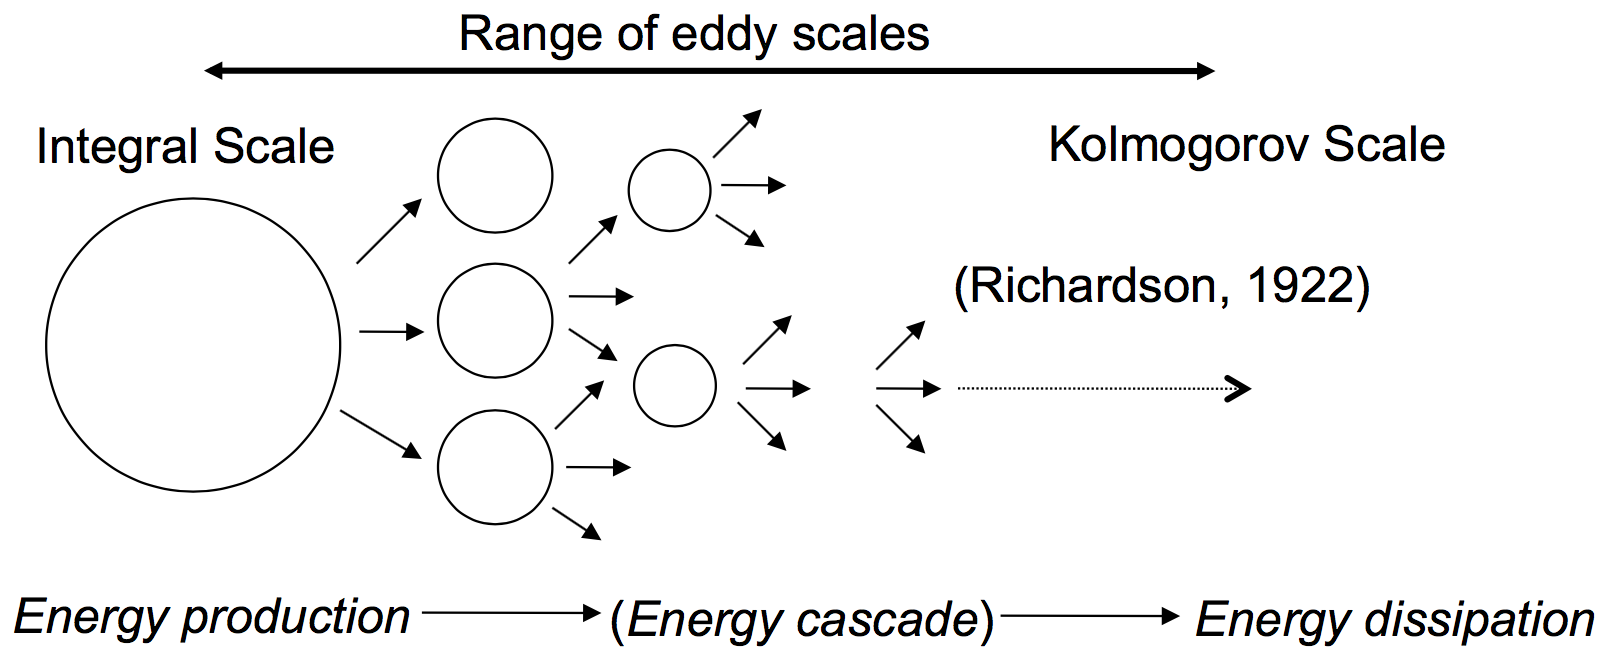
\includegraphics[width=1\textwidth]{scales.png}
\end{figure}
\end{frame}

%------------------------------------------------
\begin{frame}{Turbulent Energy Cascade}
\begin{itemize}
	\item Consider a fully developed turbulent flow at high Reynolds number
	$$\mathrm{Re} = \frac{\mathcal{U}\mathcal{L}}{\nu}$$
	where $\mathcal{U}$ is the characteristic velocity scale of the flow and $\mathcal{L}$ is the characteristic length scale of the flow.
	\item As we covered earlier in the course, we expect Re to be large for a turbulent flow (larger means a more developed flow).
	\item Let's apply the \textit{Richardson conceptual model of turbulence} to understand the flow.
\end{itemize}
\end{frame}

%------------------------------------------------

\begin{frame}{Turbulent Energy Cascade}
  
\setlength{\fboxsep}{0pt}
\setlength{\fboxrule}{1pt}
\begin{columns}[T]
    \begin{column}{.58\textwidth}
    	\begin{itemize}
    		\item Lewis Fry Richardson (1881--1953)
    		\item Pioneered the idea of predicting weather by solving differential equations.
    		\item \emph{Weather Prediction by Numerical Process} (1922)
    	\end{itemize}	
    \end{column}
    \begin{column}{.42\textwidth}
    	\begin{minipage}[c][.5\textheight][c]{\linewidth}
    		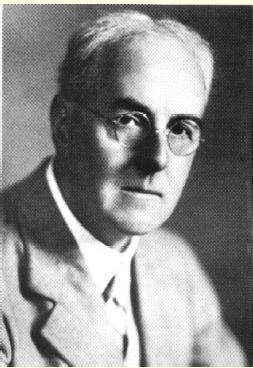
\includegraphics[width=\textwidth]{richardson.png}
    	\end{minipage}
    \end{column}
  \end{columns}
\end{frame}

%------------------------------------------------

\begin{frame}{Turbulent Energy Cascade}
	Richardson, from \emph{Weather Prediction by Numerical Process} (1922)
	\begin{fancyquotes}
		Big whorls have little whorls\\
		That feed on their velocity;\\
		And little whorls have lesser whorls\\
		And so on to viscosity.
	\end{fancyquotes}
\end{frame}

%------------------------------------------------
\begin{frame}{Turbulent Energy Cascade}
\begin{itemize}
	\item Richardson's concept of turbulence implies that the flow is composed of turbulent eddies.
	\item Consider a generic eddy of size (scale) $\ell$.
	\item This eddy will have a velocity scale $u(\ell)$ and time scale $\tau (\ell) \equiv l / u(\ell)$.
	\item The eddy is considered to be a unit carrier of turbulent motion.
	\item Furthermore, the eddy is localized within a region of size $\ell$ and assumed to be at least moderately coherent over this region.
\end{itemize}
\end{frame}

%------------------------------------------------
\begin{frame}{Turbulent Energy Cascade}
\begin{itemize}
	\item If we look at the largest eddies in the flow, they are on the scale of the flow itself.
	\item We call this largest scale the integral scale ($\ell_o \sim \mathcal{L}$), which is on the order of the auto-correlation length - or in a boundary layer, the integral scale is comparable to the boundary layer depth.
	\item The associated velocity scale $u_o(\ell_o)$ is on the order of the turbulence intensity.
	\item The Reynolds number of these eddies, Re$=u_o \ell_o/\nu$, is large relative to that of smaller eddies in the flow and is comparable to Re.	
\end{itemize}
\end{frame}

%------------------------------------------------

\begin{frame}{Turbulent Energy Cascade}
	The idea of the turbulent cascade:
	\begin{itemize}
		\item Vorticity is created on large scales by some driving mechanism that feeds energy to the fluid, which results in these large eddies.
		\item Shear instability causes smaller vortices to be shed, drawing energy from the larger ones.
		\item This process continues on ever smaller scales.
		\item On the smallest scales, diffusion destroys eddies and converts their kinetic energy to thermal energy.
	\end{itemize}
	
	\begin{figure}
		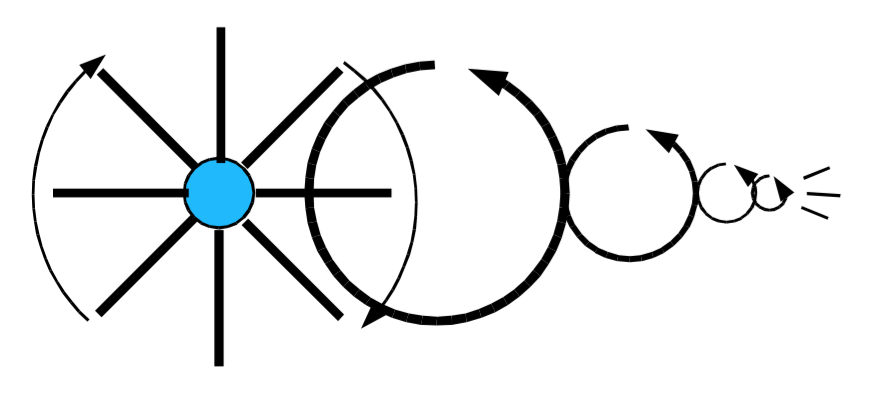
\includegraphics[width=0.5\textwidth]{scales3}
	\end{figure}
\end{frame}
%------------------------------------------------

\begin{frame}{Turbulent Energy Cascade}
	The idea of the turbulent cascade:
	\begin{itemize}
		\item The cascade is considered a closed system.
		\item The energy transfer rate (energy per unit mass per unit time) by large eddies at the start (s) of the cascade is equal to the energy transfer rate at the finish (f) of the cascade:
		$$P_s \sim \frac{u_s^2}{\tau_s} \sim \frac{u_s^2}{\ell_s / u_s} \sim \frac{u_s^3}{\ell_s} \simeq \frac{u_f^3}{\ell_f} \simeq P_f$$
	\end{itemize}
	
	\begin{figure}
		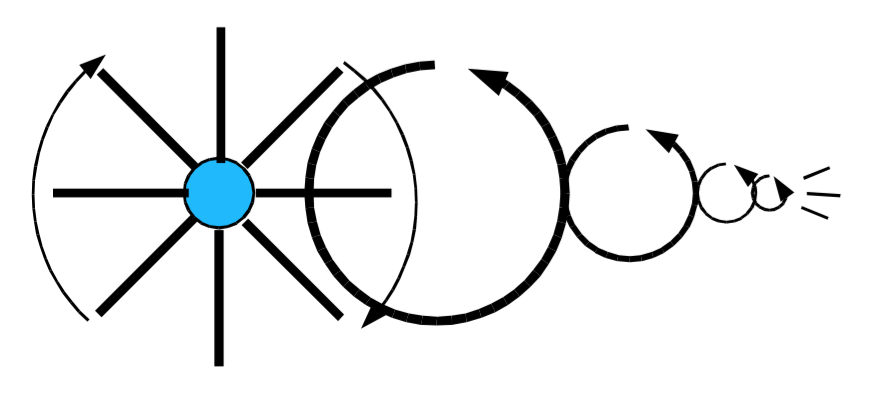
\includegraphics[width=0.5\textwidth]{scales3}
	\end{figure}
\end{frame}

%------------------------------------------------
\begin{frame}{Turbulent Energy Cascade}
\begin{figure}
	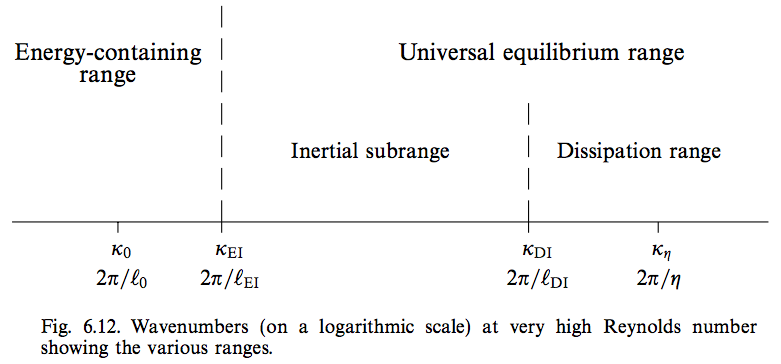
\includegraphics[width=1\textwidth]{turb1.png}
\end{figure}
\end{frame}

%------------------------------------------------
\begin{frame}{Turbulent Energy Cascade}
\begin{figure}
	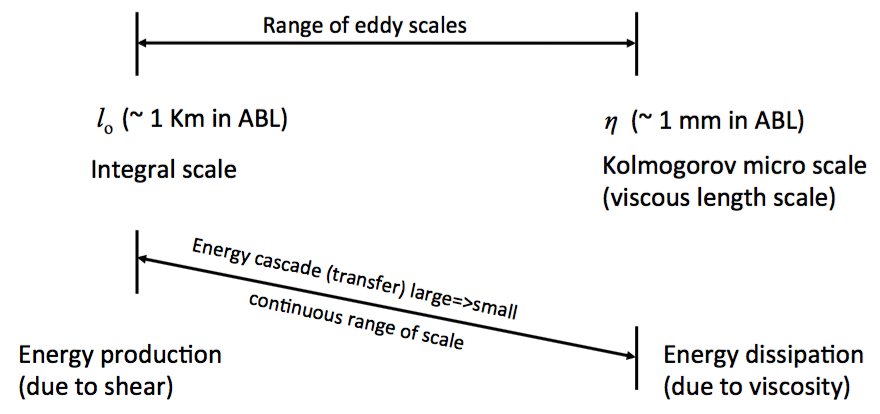
\includegraphics[width=1\textwidth]{scales2.png}
\end{figure}
\end{frame}

%------------------------------------------------

\begin{frame}{Remember da Vinci?}
  \setlength{\fboxsep}{0pt}
  \setlength{\fboxrule}{1pt}
  \begin{figure}[H]
  \centering
  \fbox{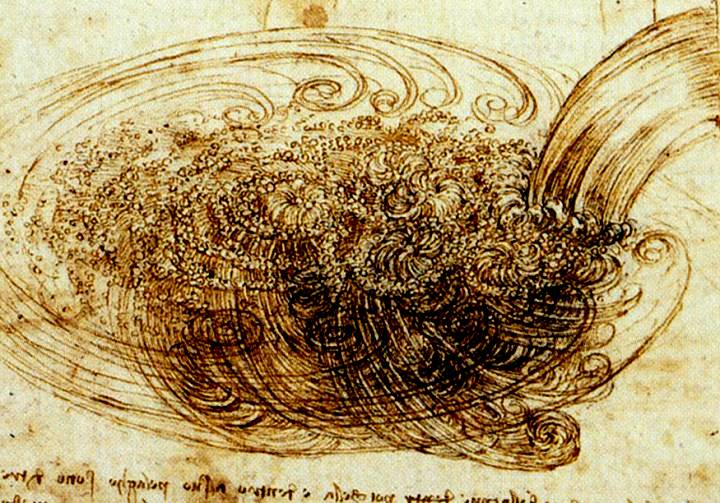
\includegraphics[width=0.5\textwidth]{davinci2.jpg}}
  \end{figure}
  
      \begin{fancyquotes}
      ... the smallest eddies are almost numberless, and large things are rotated only by large eddies and not by small ones, and small things are turned by small eddies and large.	
      \end{fancyquotes}
Sounds like Richardson's turbulent cascade!
\end{frame}
%------------------------------------------------
\section{Kolmogorov's similarity hypothesis} %
%------------------------------------------------
\framecard[colorred]{{\color{white}\Huge Kolmogorov's similarity hypothesis}}
%------------------------------------------------
\begin{frame}{Kolmogorov's similarity hypothesis (1941)}
  
\setlength{\fboxsep}{0pt}
\setlength{\fboxrule}{1pt}
\begin{columns}[T]
    \begin{column}{.58\textwidth}
    	\begin{itemize}
    		\item Andrey Nikolaevich Kolmogorov (1903--1987).
    		\item Famous Russian mathematician.
    		\item Very influential 1941 theory of homogeneous, isotropic, incompressible turbulence based on Richardson's ideas.
    	\end{itemize}	
    \end{column}
    \begin{column}{.42\textwidth}
    	\begin{minipage}[c][.5\textheight][c]{\linewidth}
    		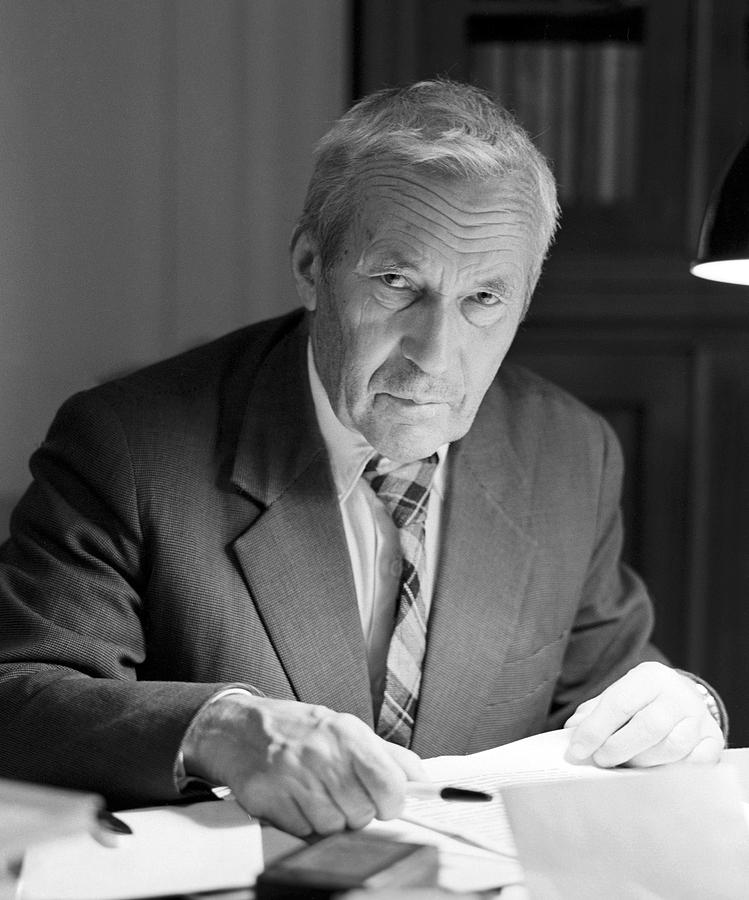
\includegraphics[width=\textwidth]{kolmogorov.jpg}
    	\end{minipage}
    \end{column}
  \end{columns}
\end{frame}

%------------------------------------------------

\begin{frame}{Kolmogorov's similarity hypothesis (1941)}
	Kolmogorov's theory of turbulence
	\begin{itemize}
		\item Turbulence displays universal properties independent of initial and boundary conditions.
		\item Energy is added to the fluid on the inertial scale $\ell_o$ and is dissipated as heat on the dissipative scale.
		\item Energy transfer between eddies on intermediate scales is lossless.
	\end{itemize}
\end{frame}

%------------------------------------------------

\begin{frame}{Kolmogorov's similarity hypothesis (1941)}
	Kolmogorov's local isotropy hypothesis
	\begin{itemize}
		\item As Re becomes large, the small-scale turbulent motions in all flows have similar universal character.
		\item These motions are assumed to be statistically isotropic (local isotropy hypothesis),
	\end{itemize}
\end{frame}

%------------------------------------------------

\begin{frame}{Kolmogorov's similarity hypothesis (1941)}
	Kolmogorov's first hypothesis
	\begin{itemize}
		\item Smallest scales receive energy at a rate proportional to the dissipation of energy rate.
		\item Motion of the very smallest scales in a flow depend only on:
		\begin{itemize}
			\item rate of energy transfer from small scales
			$$\epsilon \left[ \frac{L^2}{T^3}\right]$$
			\item kinematic viscosity
			$$\nu \left[\frac{L^2}{T} \right]$$
		\end{itemize}
	\end{itemize}
\end{frame}

%------------------------------------------------

\begin{frame}{Kolmogorov's similarity hypothesis (1941)}
	Using these, he defined the Kolmogorov scales (dissipation scales)
	\begin{itemize}
		\item length scale $$\eta = \left(\frac{\nu^3}{\epsilon}\right)^{\frac{1}{4}}$$
		\item time scale $$\tau = \left(\frac{\nu}{\epsilon}\right)^{\frac{1}{2}}$$
		\item velocity scale $$v = \frac{\eta}{\nu} = (\nu \epsilon)^{\frac{1}{4}}$$
	\end{itemize}
	Check units for yourself.
\end{frame}

%------------------------------------------------

\begin{frame}{Kolmogorov's similarity hypothesis (1941)}
\begin{itemize}
	\item Recall, that the Reynolds number (Re=$UL/\nu$) is the ratio of inertia to viscous forces.
	\item Based on the Kolmogorov scales: $$\text{Re} = \frac{v \eta}{\nu} = \frac{ (\nu \epsilon)^{\frac{1}{4}} \left(\frac{\nu^3}{\epsilon}\right)^{\frac{1}{4}}}{\nu} = \nu^{\frac{1}{4}} \epsilon^{\frac{1}{4}} \nu^{\frac{3}{4} }\epsilon^{-\frac{1}{4}} \nu^{-1} = 1$$
\end{itemize}
Or in other words, the Kolmogorov length scale is the scale at which Re=1
\end{frame}

%------------------------------------------------

\begin{frame}{Kolmogorov's similarity hypothesis (1941)}
\begin{itemize}
	\item From these scales, we can also form the ratios of the largest to smallest scales in a flow. 
	\item We will denote the largest length, time, and velocity scales as $\ell_o$, $t_o$, and $U_o$, respectively.
	\item We can approximate dissipation at large scales as $$\epsilon \sim \frac{U_o^3}{\ell_o}$$
\end{itemize}
\end{frame}

%------------------------------------------------

\begin{frame}{Kolmogorov's similarity hypothesis (1941)}
\begin{itemize}
	\item length scale
	\begin{align*} 
		\eta &= \left(\frac{\nu^3}{\epsilon}\right)^{\frac{1}{4}} \sim \left(\frac{\nu^3 \ell_o}{U_o^3}\right)^{\frac{1}{4}}\\ 
		&\Rightarrow \frac{\ell_o^{\frac{1}{4}}}{\eta} \sim \frac{U_o^{\frac{3}{4}}}{\nu^{\frac{3}{4}}}\\
		&\Rightarrow \frac{\ell_o}{\eta} \sim \frac{U_o^{\frac{3}{4}}\ell_o^{\frac{3}{4}}}{\nu^{\frac{3}{4}}} \\
		\Aboxed{&\Rightarrow \frac{\ell_o}{\eta} \sim \text{Re}^{\frac{3}{4}}}
	\end{align*}
\end{itemize}
\end{frame}

%------------------------------------------------

\begin{frame}{Kolmogorov's similarity hypothesis (1941)}
\begin{itemize}
	\item velocity scale
	\begin{align*} 
		v &= \frac{\eta}{\nu} \sim \left( \frac{\nu U_o^3}{\ell_o}\right)^{\frac{1}{4}}\\
		&\Rightarrow \frac{U_0^{\frac{3}{4}}}{v} \sim \frac{\ell_o^{\frac{1}{4}}}{\nu^{\frac{1}{4}}}\\
		&\Rightarrow \frac{U_0}{v} \sim \frac{U_o^{\frac{1}{4}}\ell_o^{\frac{1}{4}}}{\nu^{\frac{1}{4}}}\\
		\Aboxed{ &\Rightarrow \frac{U_0}{v} \sim \text{Re}^{\frac{1}{4}}}
	\end{align*}
\end{itemize}
\end{frame}

%------------------------------------------------

\begin{frame}{Kolmogorov's similarity hypothesis (1941)}
\begin{itemize}
	\item time scale
	\begin{align*} 
		\tau &= \frac{\eta}{v}\\
		&\Rightarrow \frac{t_o}{\tau} = \frac{\ell_o/U_o}{\eta/v}\\
		&\Rightarrow \frac{t_o}{\tau} = \left(\frac{\ell_o}{\eta}\right) \left(\frac{U_o}{v}\right)^{-1}\\
		&\Rightarrow \frac{t_o}{\tau} \sim \text{Re}^{\frac{3}{4}} \text{Re}^{-\frac{1}{4}}\\
		\Aboxed{&\Rightarrow \frac{t_o}{\tau} \sim \text{Re}^{\frac{1}{2}}}
	\end{align*}
\end{itemize}
\end{frame}

%------------------------------------------------

\begin{frame}{Kolmogorov's similarity hypothesis (1941)}
\begin{itemize}
	\item For very high-Re flows (\textit{e.g.}, Atmosphere), we have a range of scales that is small compared to $\ell_o$ but large compared to $\eta$.
	\item As Re increases, $\ell_o/\eta$ increases. This results in a larger separation of between large and small scales.
\end{itemize}
\end{frame}

%------------------------------------------------

\begin{frame}{Kolmogorov's similarity hypothesis (1941)}
\begin{itemize}
	\item Consider typical atmospheric scales:$$U_o\sim10\ \metre\ \reciprocal\second,\ \ell_o\sim10^3\ \metre,\ \nu \sim 10^{-5}\ \square\metre\ \reciprocal\second$$
	\item which gives us, $$\text{Re} = \frac{U_o \ell_o}{\nu} \sim \frac{(10\ \metre\ \reciprocal\second)(10^3\ \metre)}{10^{-5}\ \square\metre\ \reciprocal\second} \sim 10^9$$
	\item thus, 
	\begin{align*}
		\eta &\sim \ell_o \text{Re}^{-\frac{3}{4}} \sim 0.00018\ \metre \\
		v &\sim U_o \text{Re}^{-\frac{1}{4}} \sim 0.06\ \metre\ \reciprocal\second \\
		\tau &\sim \frac{\ell_o}{U_o} \text{Re}^{-\frac{1}{2}} \sim 0.003\ \second
	\end{align*}
\end{itemize}
You can start to see why explicitly resolving all scales in a typical atmosphere is expensive!
\end{frame}

%------------------------------------------------

\begin{frame}{Kolmogorov's similarity hypothesis (1941)}
	Kolmogorov's second hypothesis
	\begin{itemize}
		\item In turbulent flow, a range of scales exists at very high Re where statistics of motion in a range $l$ ($\ell_o \gg \ell \gg \eta$) have a universal form that is determined only by $\epsilon$ (dissipation) and independent of $\nu$ (kinematic viscosity).
		\item Kolmogorov formed his hypothesis and examined it by looking at the PDF of velocity increments $\Delta u$.
	\end{itemize}
\end{frame}

%------------------------------------------------

\begin{frame}{Kolmogorov's similarity hypothesis (1941)}
	Kolmogorov's second hypothesis
	\begin{itemize}
		\item Using dimensional analysis (Buckingham Pi), we have that the spectral energy density, $[L^3/T^2]$, is a function of only wavenumber $k = 2\pi/\ell$, $[1/L]$, and dissipation $\epsilon$, $[L^2/T^3]$:
		\item We arrive at:
		 $$E(K) = c_k \epsilon^{2/3}k^{-5/3}$$
		 where $c_k$ is the Kolmogorov ``constant'' and is assumed to be around 1.5 or so.
		 \item This is the famous Kolmogorov's -5/3 power law.
	\end{itemize}
\end{frame}

%------------------------------------------------
\begin{frame}{Kolmogorov's similarity hypothesis (1941)}
\begin{figure}
	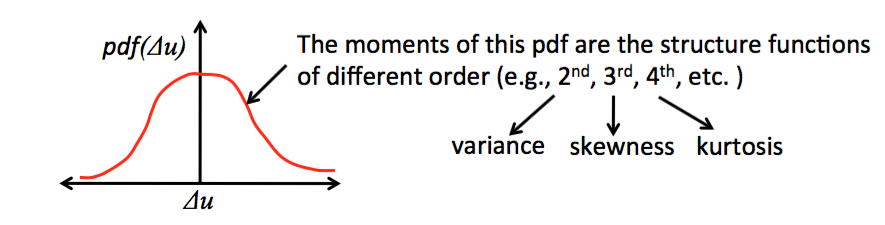
\includegraphics[width=1\textwidth]{pdf.png}
\end{figure}
What are structure functions? The PDF? Let's quickly recap statistics and how they tie in to scales.
\end{frame}


%------------------------------------------------
\begin{frame}{Stats review}
\begin{itemize}
	\item The PDF is the integral of the CDF	
	\item It gives the probability per unit distance in the sample space -- hence, the term \textit{density}
	\item If two or more signals have the same PDF, then they are considered to be statistically identical.
	\item Practically speaking, we find the PDF of a time (or space) series by:
	\begin{itemize}
  	\item Create a histogram of the series(group values into bins)
  	\item Normalize the bin weights by the total \# of points
  \end{itemize}
\end{itemize}

\end{frame}

%------------------------------------------------
\begin{frame}{Stats review}
\textit{Autocovariance} measures how a variable changes with different lags, $s$.
  $$R(s) \equiv \langle u(t) u(t+s)\rangle$$
  or the \textit{autocorrelation function}
  $$\rho(s) \equiv \frac{ \langle u(t)u(t+s)\rangle}{u(t)^2}$$
  Or for the discrete form
  $$\rho(s_j) \equiv \frac{ \sum^{N-j-1}_{k=0}(u_ku_{k+j})}{\sum^{N-1}_{k=0}(u_k^2)}$$
\end{frame}

%------------------------------------------------

\begin{frame}{Stats review}
  
  Notes on autocovariance and autocorrelation
  \begin{itemize}
  	\item These are very similar to the covariance and correlation coefficient
  	\item The difference is that we are now looking at the linear correlation of a signal with itself but at two different times (or spatial points), i.e. we lag the series.
  	\item We could also look at the cross correlations in the same manner (between two different variables with a lag).
  	\item $\rho(0) = 1$ and $|\rho(s)| \leq 1$
  \end{itemize}
  
\end{frame}

%------------------------------------------------

\begin{frame}{Stats review}
    \begin{itemize}
    	\item In turbulent flows, we expect the correlation to diminish with increasing time (or
distance) between points
    	\item We can use this to define an integral time (or space) scale. It is defined as the time lag where the integral $\int \rho(s)ds$ converges. 
    	\item It can also be used to define the largest scales of motion (statistically).
    \end{itemize}
  
  \begin{figure}
  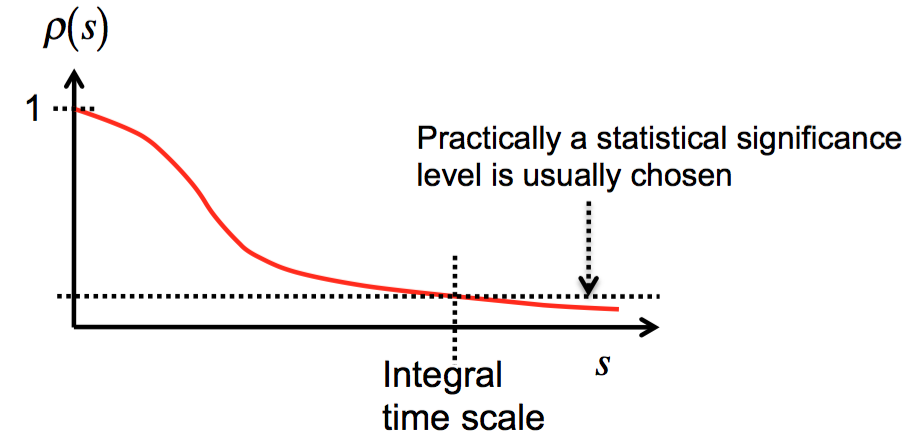
\includegraphics[width=0.8\textwidth]{auto1.png}
  \end{figure}
  
\end{frame}

%------------------------------------------------

\begin{frame}{Stats review}
  
  The \textit{structure function} is another important two-point statistic.
  $$D_n(r) \equiv \langle [U_1(x+r,t) - U_1(x,t)]^n\rangle$$
  \begin{itemize}
  	\item This gives us the average difference between two points separated by a distance $r$ raised to a power $n$.
  	\item In some sense it is a measure of the moments of the velocity increment PDF.
  	\item Note the difference between this and the autocorrelation which is statistical linear correlation (\textit{i.e.}, multiplication) of the two points.
  \end{itemize}
  
\end{frame}

%------------------------------------------------
\section{Fourier transforms} %
%------------------------------------------------
\begin{frame}{Fourier transforms}
Alternatively, we can also look at turbulence in wave (frequency) space. \textbf{Fourier transforms} are a common tool in fluid dynamics (see Pope, Appendix D-G, Stull handouts online).\newline\newline
Some uses:
\begin{itemize}
	\item Analysis of turbulent flow
	\item Numerical simulations of N-S equations
	\item Analysis of numerical schemes (modified wavenumbers)
\end{itemize}
\end{frame}

%------------------------------------------------
\begin{frame}{Fourier transforms}

\begin{itemize}
	\item Consider a periodic function $f(x)$ [could also be $f(t)$] on a domain of length $2\pi$.	
	\item The Fourier representation of this function (or a general signal) is:
	$$f(x) = \sum^{k=\infty}_{k=-\infty} \hat f_k e^{ikx}$$
	where $k$ is the wavenumber (frequency if $f(t)$), and $\hat f_k$ are the Fourier coefficients which in general are complex.
\end{itemize}
\end{frame}

%------------------------------------------------
\begin{frame}{Fourier transforms}

Why pick $e^{ikx}$?
\begin{itemize}
	\item Orthogonality $$\int^{2\pi}_{0} e^{i(k-k^\prime)x} dx = \begin{cases}
    0,& \text{if } k\neq k^\prime\\
    2\pi & \text{if } k=k^\prime
\end{cases}$$
	\item a big advantage of orthogonality is independence between Fourier modes
	\item $e^{ix}$ is independent of $e^{i2x}$, just like we have with Cartesian coordinates -- where $i,j,k$ are all independent of each other
	\end{itemize}
\end{frame}

%------------------------------------------------
\begin{frame}{Fourier transforms}

What are we doing?
\begin{itemize}
	\item Recall from Euler's formula that $e^{ix}$ = $\cos (x) - i\sin (x)$
	\item The Fourier transform decomposes a signal (space or time) into sine and cosine wave components of different amplitudes and wave numbers (or frequencies).
	\end{itemize}
\end{frame}

%------------------------------------------------
\begin{frame}{Fourier transforms}

Fourier transform example (from Stull, see FourierTransDemo.m)
\begin{figure}
	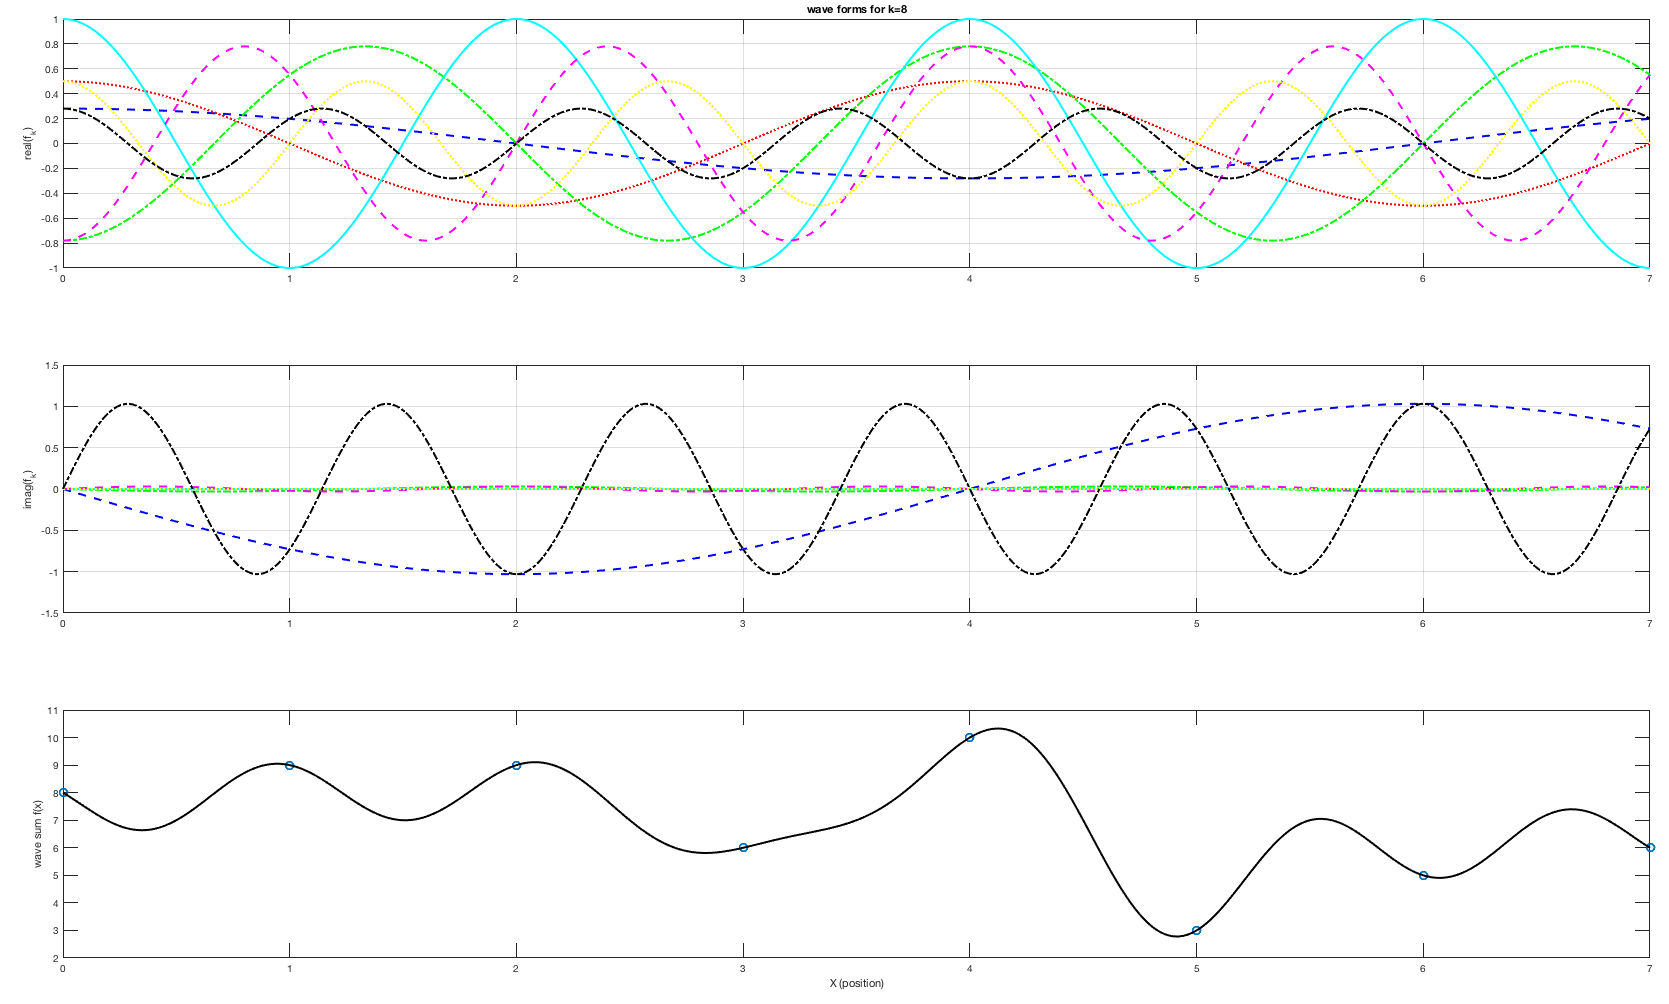
\includegraphics[width=\textwidth]{fourier.png}
\end{figure}
\end{frame}

%------------------------------------------------
\begin{frame}{Fourier transforms}

\begin{itemize}
	\item The Fourier representation below is a representaion of a series as a function of sine and cosine waves. It takes $f(x)$ and transforms it into wave space.
	\item Fourier transform pair: consider a periodic function on a domain of $2\pi$
	\begin{align*}
		f_k &= F\{f(x)\} \equiv \frac{1}{2\pi} \int^{2\pi}_{0} f(x) e^{-ikx}dx &\rightarrow & \text{ forward transform}\\
		f(x) &= F\{\hat f_k\}^{-1} \equiv \sum^{k=\infty}_{k=-\infty} \hat f_k e^{ikx} &\rightarrow & \text{ backward transform}
	\end{align*}
	\item The forward transform moves us into Fourier (or wave) space and the backward transform moves us from wave space back to real space.
	\end{itemize}
\end{frame}


%------------------------------------------------
\begin{frame}{Fourier transforms}

An alternative form of the Fourier transform (using Euler's) is:
$$f(x) = a_0 + \sum^{k=\infty}_{k=-\infty} a_k\cos(kx) - b_k\sin{kx}$$
where $a_k$ and $b_k$ are the real and imaginary components of $f_k$, respectively.

\end{frame}

%------------------------------------------------
\begin{frame}{Fourier transform properties}

\begin{itemize}
	\item if $f(x)$ is real, then: $$\hat f_k = \hat f_kA^*$$
	\item Parseval's Theorem: $$\frac{1}{2\pi} \int^{2\pi}_{0} f(x) f^*(x)dx = \sum^{k=\infty}_{k=-\infty} \hat f_k \hat f_k^*$$
	\item The Fourier representation is the best possible representation for $f(x)$ in the sense that the error:
	$$\text{e} = \int^{2\pi}_{0} \left| f\left(x - \sum^N_{k=-N} c_k e^{ikx}\right)\right|^2 dx$$
	is a minimum when $c_k = \hat f_k$
\end{itemize}

\end{frame}

%------------------------------------------------
\begin{frame}{Discrete Fourier transform}

\begin{itemize}
	\item Consider the periodic function $f_j$ on the domain $0\leq x \leq L$ (periodicity implies that $f(0) = f(N)$) \begin{figure}
		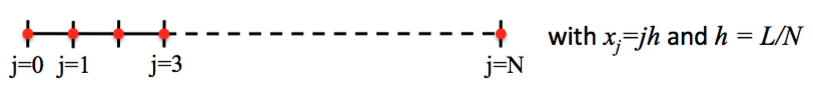
\includegraphics[width=0.9\textwidth]{discrete1.png}	
	\end{figure}
	\item Discrete Fourier representation:$$f_j = \sum_{k=-N/2}^{N/2-1} \hat f_k e^{i\frac{2\pi}{L}kx_j}\ \Rightarrow \text{backward (inverse) transform}$$
	We know $f_j$ at $N$ pts, don't know $\hat f_k$ at $k$ values ($N$ of them).
 	\item Using discrete orthogonality:$$\hat f_k = \frac{1}{N} \sum_{j=0}^{N-1} f_j e^{-i\frac{2\pi}{L}kx_j}\ \Rightarrow \text{forward transform}$$
 	
\end{itemize}
\end{frame}

%------------------------------------------------
\begin{frame}{Discrete Fourier transform}

\begin{itemize}
	\item Discrete Fourier Transform (DFT) example and more explanation found on the website/Canvas (Stull, Chapter 8.4--8.6., Pope appendix F, FourierTransDemo.m).
	\item Implementation of DFT by brute force $\rightarrow \mathcal{O}(N^2)$ operations.
	\item In practice, we almost always use a Fast Fourier Transform (FFT) $\rightarrow \mathcal{O}(N\log_2 N)$ operations.
\end{itemize}
\end{frame}

%------------------------------------------------
\begin{frame}{Discrete Fourier transform}

\begin{itemize}
	\item Almost all FFT routines (\textit{e.g.}, Matlab, FFTW, Intel, Numerical Recipes, etc.) save their data with the following format:
	\begin{figure}
		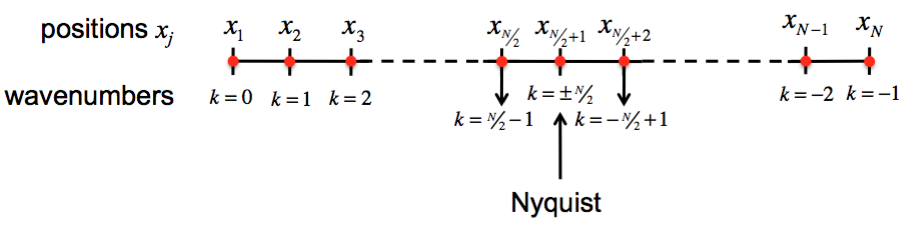
\includegraphics[width=0.9\textwidth]{discrete2.png}	
	\end{figure}
\end{itemize}
\end{frame}

%------------------------------------------------
\begin{frame}{Fourier transform applications: autocorrelation}

Autocorrelation
\begin{itemize}
	\item We can use the discrete Fourier Transform to speed up the autocorrelation calculation (or in general any cross-correlation with a lag). Discretely,$$R_{ff} (s_l) = \sum^{N-1}_{j=0} f(x_j) f(x_j + s_l)\ \Rightarrow \mathcal{O}(N^2) \text{operations}$$
	\item If we express $R_{ff}$ as a Fourier series$$R_{ff}(s_l) = \sum\nolimits_{k}  \hat R_{ff} e^{iks_l} \Rightarrow R_ff(0) = \sum_k \hat R_{ff}$$
	and we can show that $$R_{ff}(0) = \sum\nolimits_{k}  N\underbrace{|\hat f_k|^2}_{\mathclap{\substack{\text{magnitude of}\\\text{Fourier Coefficients}} }}$$
\end{itemize}

\end{frame}

%------------------------------------------------
\begin{frame}{Fourier transform applications: autocorrelation}

How can we interpret this?
\begin{itemize}
	\item In physical space
	\begin{align*}
	R_{ff}(0) &= \sum^{N-1}_{j=0} f_j^2\ (\text{\emph{i.e.}, the mean variance})\\
	&\Rightarrow \sum^{N-1}_{j=0} f_j^2 = \sum_{k=-N/2}^{N/2-1} \underbrace{N|\hat f_k|^2}_{\mathclap{\substack{\text{energy}\\\text{spectral density}} }}\}{\substack{\text{total contribution}\\\text{to the variance}}}
	\end{align*}
\end{itemize}

\end{frame}


%------------------------------------------------
\begin{frame}{Fourier transform applications: spectrum}

Energy Spectrum: (power spectrum, energy spectral density)
\begin{itemize}
	\item If we look at specific $k$ values from we can define: $$E(k) = N|\hat f_k|^2$$ where $E(k)$ is the energy spectral density
	\item  The square of the Fourier coefficients is the contribution to the variance by fluctuations of scale $k$ (wavenumber or equivalently frequency)
	\item Typically (when written as) $E(k)$ we mean the contribution to the turbulent kinetic energy (TKE) = $0.5(u^2+v^2+w^2)$ and we would say that $E(k)$ is the contribution to TKE for motions of the scale (or size) $k$ . For a single velocity component in one direction we would write $E_{11}(k_1)$.
\end{itemize}

\end{frame}

%------------------------------------------------
\begin{frame}{Fourier transform applications: spectrum}

Example energy spectrum
\begin{figure}
	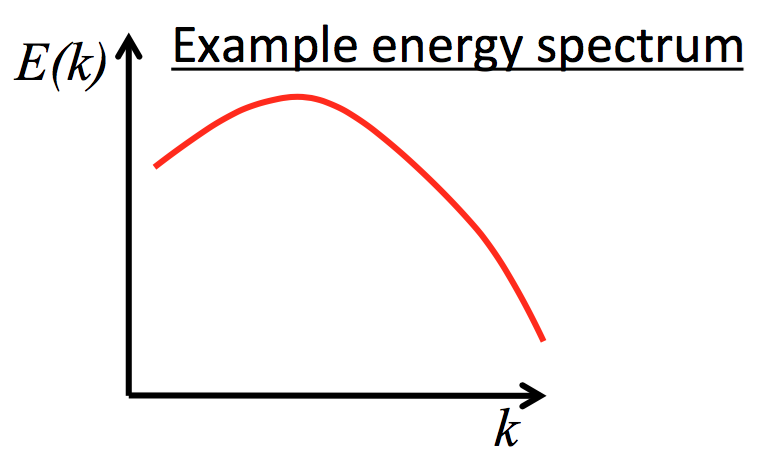
\includegraphics[width=\textwidth]{spectrum1.png}
\end{figure}
\end{frame}

%------------------------------------------------
\begin{frame}{Spectrum: sampling theorem}
\begin{itemize}
	\item \underline{Band-Limited function}: a function where $\hat f_k = 0$ for $|k| > k_c$.
	\begin{figure}
		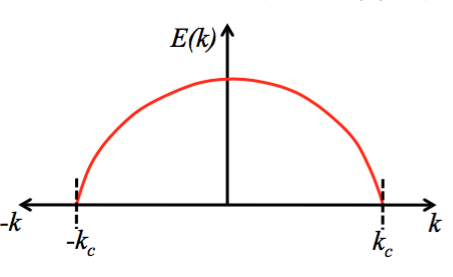
\includegraphics[width=0.8\textwidth]{sampling1.png}
	\end{figure}
\end{itemize}
\end{frame}

%------------------------------------------------
\begin{frame}{Spectrum: sampling theorem}
\begin{itemize}
	\item \underline{Theorem}: if $f(x)$ is band-limited, then $f(x)$ is completely represented by its values on a discrete grid, $x_n = n\pi/k_c$, where $n$ is an integer ($\infty < n < \infty$) and $k_c$ is called the Nyquist frequency.
	\begin{figure}
		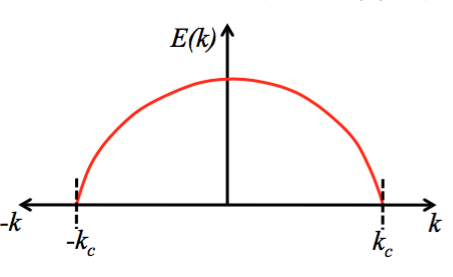
\includegraphics[width=0.8\textwidth]{sampling1.png}
	\end{figure}
\end{itemize}
\end{frame}

%------------------------------------------------
\begin{frame}{Spectrum: sampling theorem}
\begin{itemize}
	\item \underline{Implication}: if we have $x_j = j\pi/k_c = jh$ ($h = \pi/k_c$) with a domain of $2\pi$, then $h=2\pi/N = \pi/k_c \Rightarrow k_c = N/2$
	\item If the number of points is $\geq 2k_c$, then the \textit{discrete Fourier transform is the exact solution}. For example, if $f(x)=\cos (6x)$, then we need $N \geq 12$ points to represent the function exactly.
	\begin{figure}
		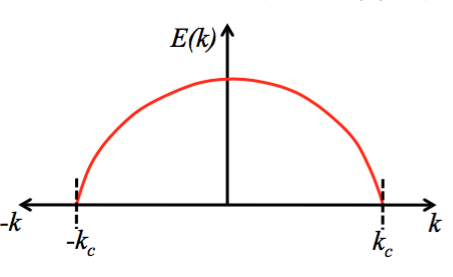
\includegraphics[width=0.8\textwidth]{sampling1.png}
	\end{figure}
\end{itemize}
\end{frame}

%------------------------------------------------
\begin{frame}{Spectrum: sampling theorem}
\begin{itemize}
	\item What if $f(x)$ is not band-limited?
	\item What if $f(x)$ is band-limited, but sampled at a rate $< k_c$ (\textit{e.g.}, $f(x)=cos(6x)$ with 8 points)?
	\begin{figure}
		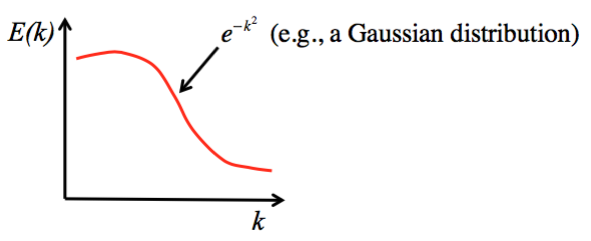
\includegraphics[width=0.8\textwidth]{sampling2.png}
	\end{figure}
	\item The result is \underline{aliasing} $\rightarrow$ contamination of resolved energy by energy outside of the resolved scales.
\end{itemize}
\end{frame}

%------------------------------------------------
\begin{frame}{Spectrum: aliasing}
\begin{itemize}
	\item Consider $e^{ik_1x_j}$ and $e^{ik_2x_j}$ and let $k_1 = k_2+ 2mk_c$, where $k_c$ is the Nyquist frequency, $m = \pm$ any integer, and $x_j=j\pi/k_c$:
	\begin{align*}
		e^{ik_1x_j}	&= e^{i(k_2 + 2mk_c)x_j}\\
		&= e^{ik_2x_j} e^{2m k_c x_j}\\
		&= e^{ik_2x_j} e^{2m k_c j\pi/k_c}\\
		&= e^{ik_2x_j} \underbrace{e^{i2\pi mj}}_{\mathrlap{\text{=1, integer fn of $2\pi$}}}\\
		e^{ik_1x_j} &= e^{ik_2x_j}
	\end{align*}
	The result is that we cannot distinguish between $k_2$ and $k_1 = k_2+ 2mk_c$ on a discrete grid. $k_1$ is \textit{aliased} onto $k_2$.
\end{itemize}
\end{frame}

%------------------------------------------------
\begin{frame}{Spectrum: aliasing}
\begin{itemize}
\item What does this mean for spectra?
\begin{figure}
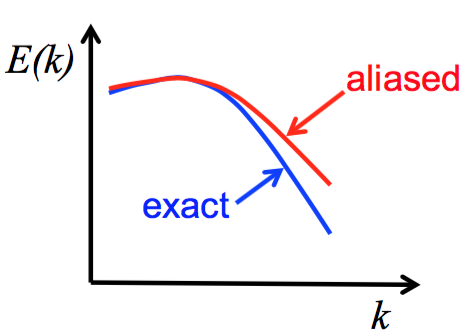
\includegraphics[width=0.4\textwidth]{alias1.png}\\
\end{figure}
\item What is actually happening?
\begin{figure}
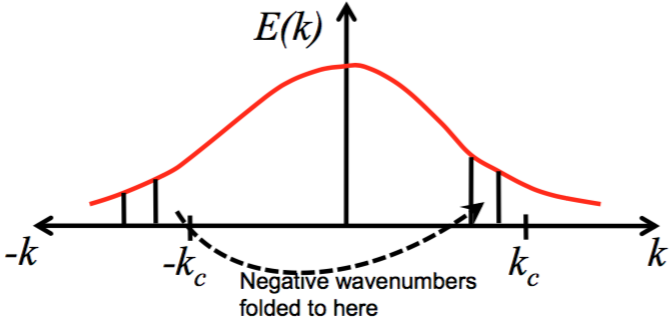
\includegraphics[width=0.6\textwidth]{alias2.png}	
\end{figure}
\end{itemize}
\end{frame}

%------------------------------------------------

\begin{frame}{Spectrum: aliasing}
Consider a function: $f(x) = \cos(x) + 0.5\cos(3x) + 0.25\cos(6x)$
\begin{itemize}
\item Fourier coefficients (all real)
\begin{figure}
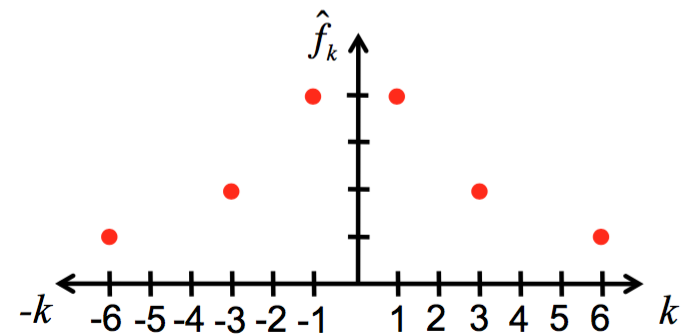
\includegraphics[width=0.4\textwidth]{alias3.png}\\
\end{figure}
\item Consider $N=8 \rightarrow k_c=4$
\begin{figure}
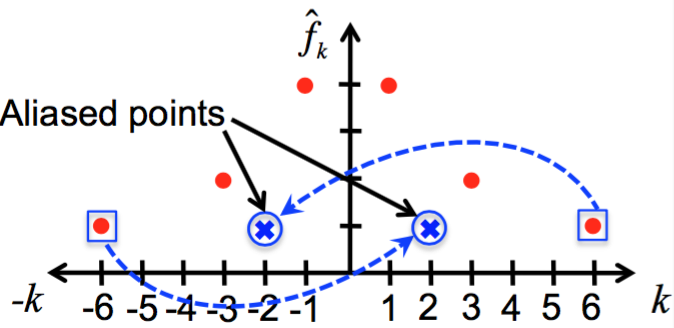
\includegraphics[width=0.4\textwidth]{alias4.png}	
\end{figure}
\item Aliasing, if $m=1$, $\Rightarrow k_1 = k_2 + 2mk_c = k_2 + 8m \Rightarrow -6$ gets aliased to 2. If $m=-1, k_1 = k_2-8 \Rightarrow 6$ gets aliased to $-2$.
\end{itemize}
\end{frame}

%------------------------------------------------

\begin{frame}{Spectrum: aliasing}
\begin{itemize}
	\item Aliasing decreases if $N$ (sampling rate) increases.
	\item For more on Fourier Transforms see Pope Ch. 6, online handout from Stull, or Press et al., Ch 12-13.
\end{itemize}
\end{frame}

%------------------------------------------------
\begin{frame}{Spectrum and Kolmogorov}

Back to Kolmogorov
\begin{itemize}
	\item Another way to look at this (equivalent to structure functions) is to examine what it means for $E(k)$ where $E(k)dk =$TKE contained between $k$ and $k+dk$.
	\item What are the implications of Kolmogorov’s hypothesis for $E(k)$? -- K41$\Rightarrow E(k) = f(k,\epsilon)$
	\item By dimensional analysis we can find that: $$E(K) = c_k \epsilon^{2/3}k^{-5/3}$$ Kolmogorov's 5/3 power law.
	\item This expression is valid for the range of length scales $\ell$ where $\ell_o \gg \ell \gg \eta$ and is usually called the inertial subrange of turbulence.
\end{itemize}
\end{frame}

%------------------------------------------------
\begin{frame}{Spectrum and Kolmogorov}

Example energy spectrum
\begin{figure}
	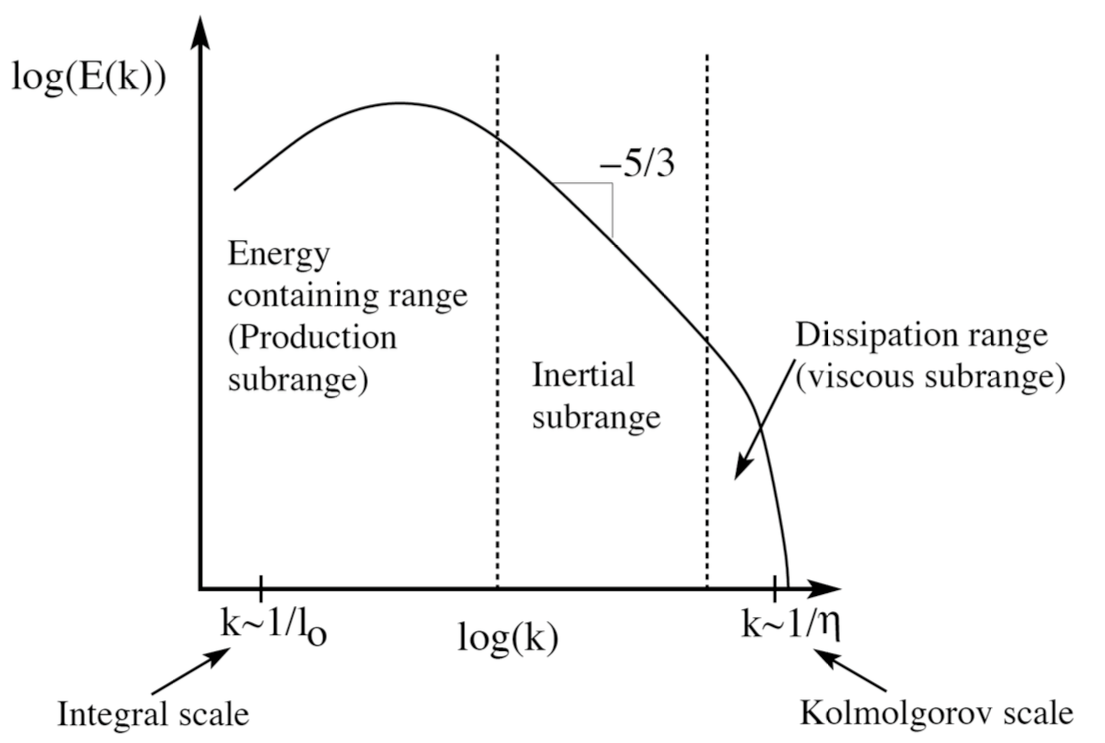
\includegraphics[width=\textwidth]{spectrum2.png}
\end{figure}
\end{frame}

%------------------------------------------------
\end{document}

